\chapter{Implémentation des premiers réseaux}

Ce chapitre décrit l'implémentation de nos réseaux de neurones sous forme de perceptrons, que nous utiliserons par la suite dans les différentes applications. Nous verrons ici cette implémentation et le premier exemple avec le XOR.

\section{Implémentation du perceptron}

\subsection{Présentation et diagramme UML}

Comme décrit dans la partie théorique sur les perceptrons (1.5), nous avons choisi de représenter nos réseaux de neurones sous forme matricielle. Les neurones ne seront donc pas représentés individuellement, mais par couche de neurones (neuronLayer). Cela permet d'effectuer les calculs sous forme matricielle par rapport à des propagations et rétro-propagations neurone par neurone, ce qui fait gagner beaucoup de temps de calcul.
Cela est possible en gardant les mêmes fonctions d'activation pour chaque neurone d'une même couche, ainsi que les mêmes entrées et sorties. Dans le cadre du perceptron, cela convient.

Le diagramme UML comporte une classe principale, Application, qui va gérer les expériences et réseaux de neurones. Cette classe contient un réseau de neurones (NeuralNetwork) composé de plusieurs couches de neurones (NeuronLayer). Application possède aussi un collecteur qui est utilisé pour récupérer les données des expériences, les traiter et les exporter dans un fichier .csv. Enfin, la classe Teacher a pour rôle de gérer la rétropropagation et l'apprentissage du réseau de neurones.

\newpage

\begin{figure}[h]
\begin{center}
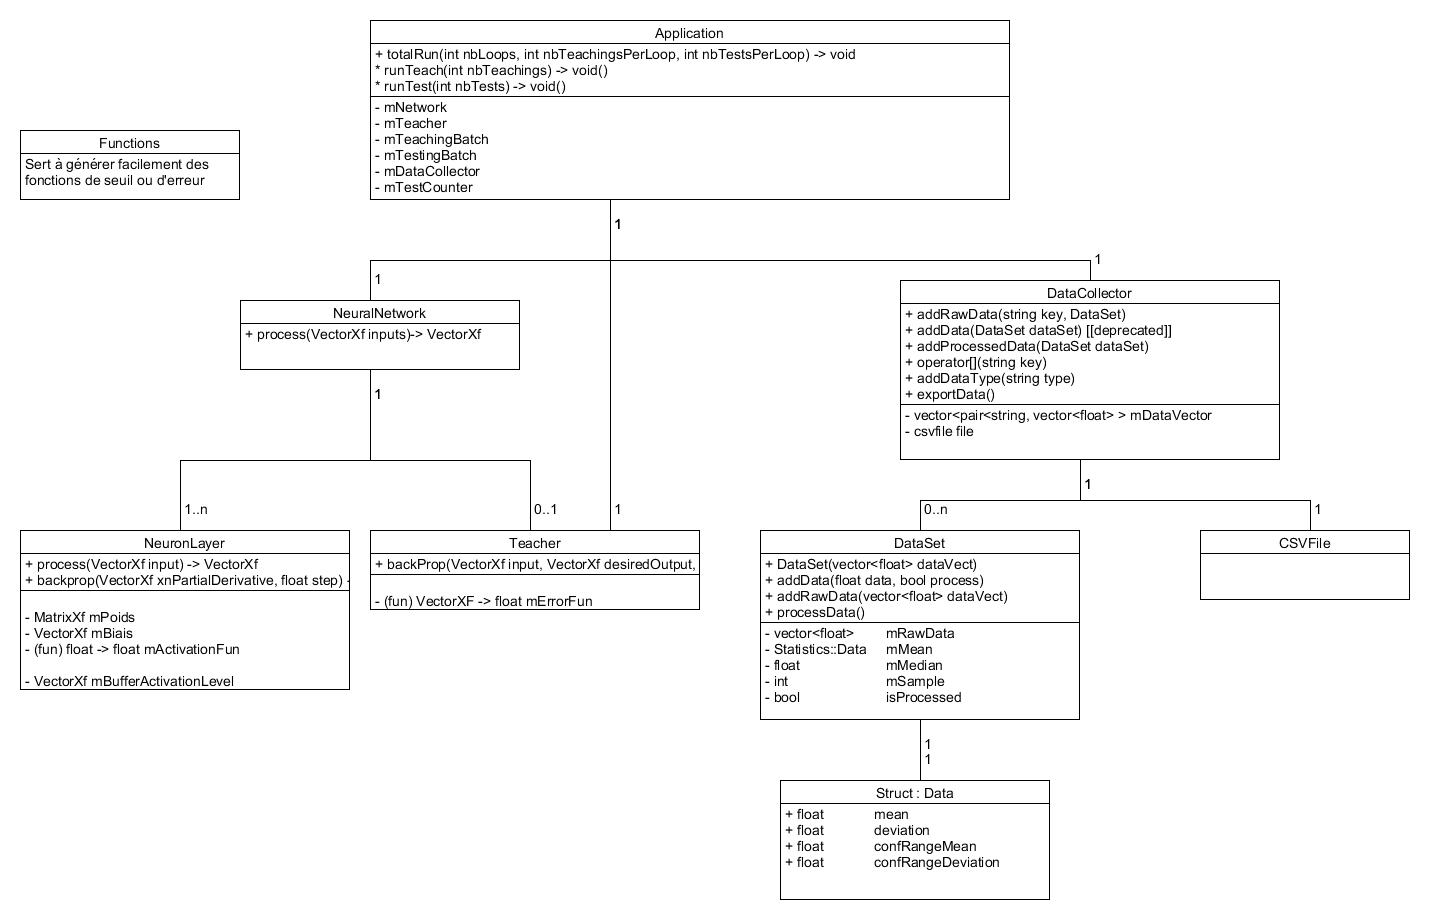
\includegraphics[width=1\textwidth]{images/umlDiagram.jpg}\caption{Diagramme UML}
\end{center}
\end{figure} 

\subsection{NeuronLayer}

Une instance de la classe \textbf{NeuronLayer} représente une couche de neurones. Comme nous utilisons la représentation matricielle des réseaux perceptrons, une couche de neurones n'est constituée que d'une matrice de poids, d'un vecteur de biais et d'une fonction d'activation. Si $input$ et $output$ représentent respectivement la dimension du vecteur d'entrée et de sortie de la couche, alors on a les dimensions suivantes (on travaille en ligne) :
\begin{itemize}
	\item La matrice de poids est de dimension $input \times output$
	\item Le vecteur de biais est un vecteur ligne de dimension $output$
\end{itemize}

\subsection{NeuralNetwork}

Une instance de la classe \textbf{NeuralNetwork} représente un réseau perceptron, c'est à dire plusieurs couches de neurones ( \texbf{NeuronLayer}) mises les unes à la suite des autres. Chaque couche de neurones reçoit en entrée la sortie de la couche précédente et transmet sa sortie à la couche suivante. 
Pour représenter cet objet, nous avons utilisé la structure de liste simplement chaînée. La class \textbf{NeuralNetwork} hérite donc de la classe \textbf{std::list<NeuronLayer>}. Cette structure légère et robuste permet d'itérer facilement sur toutes les couches du réseau. 

\subsection{DataCollector}

Afin de collecter les données du réseau et de pouvoir effectuer un traitement statistique dessus (calcul de moyenne, ecart-type, intervalle de confiance...) nous avons écrit la classe \textbf{DataCollector}. Elle se charge de récupérer les sorties du réseau, d'effectuer des calculs statistiques standards et de les exporter au format \textbf{.csv} afin de permettre une visualisation facile de toutes les données.

\section{Etude du XOR}

Le problème du XOR est un problème de classification standard, auquel toutes les méthodes de classification sont confrontées. Nous avons donc naturellement commencé par le traitement de ce problème pour nous exercer à la manipulation des perceptrons.

\subsection{Definition du problème}

Le problème du XOR est un problème en deux dimensions : les entrées sont des paires $(x_1,\ x_2)$ et la sortie est un booléen. Deux approches différentes existent, selon le choix du domaine de définition : 

\begin{itemize}
  \item 1\textsuperscript{er} choix : on veut obtenir un XOR purement booléen, dont les 4 entrées possibles sont les paires $(0,0)\ (0,1),\ (1,0),\ (1,1)$. Les résultats attendus sont respectivements $0,\ 1,\ 1,\ 0$.
  \item 2\textsuperscript{nd} choix : on veut obtenir un XOR défini sur le carré unité du plan : ${(x,y) \in [-1,1]^2}$. Dans ce cas, on attend du XOR qu'il renvoie $1$ lorsque $x \times y < 0$ et $0$ sinon. On fait donc un XOR sur le signe des coordonnées.
\end{itemize}

Selon l'approche, le réseau requis sera différent. Dans le premier cas, il est possible de classifier les 4 points selon leur appartenance à un ensemble convexe (qui prend la forme d'une bande). Par conséquent, le problème peut se résoudre avec deux couches de neurones.

Dans le second cas, il faut séparer le plan en 4 quadrants, et regrouper les quadrants par deux. On obtient des classes non convexes, et le problème requiert 3 couches de neurones pour être résolu.

Nous avons choisi de travailler sur la deuxième situation, le but est donc d'obtenir un réseau qui découpe le carré unité en quatre quadrants bien distincts, qui correspondent aux quatre quadrants délimités par les axes des abscisses et des ordonnées.

\subsection{Résolution}

Il s'agit d'un problème à deux dimensions, renvoyant une seule valeur, et nécessitant 3 couches cachées. Nous optons donc pour un réseau 2-2-1. 

Qualitativement, on peut dire que 
\begin{itemize}
  \item les deux neurones de la première couche vont se charger de tracer les deux droites correspondant aux abscisses et aux ordonnées
  \item les deux neurones de la seconde couche vont se charger de réaliser les fonctions \"ou\" et \"et\" sur les quadrants ainsi tracés, afin de d'obtenir deux quadrants correspondants au résultat $1$ et deux quadrants correspondants aux résultat $0$.
  \item la troisième couche se charge de réaliser la fonction \"ou\" sur les résultats renvoyés par la couche 2, afin que le résultat final soit $1$ si le point se trouve dans l'un des deux quadrants correspondant au résultat $1$.
\end{itemize}

De plus, nous avons choisi d'utiliser des fonctions d'activations sigmoides en $\frac{1}{1+exp(-\lambda x}$. Une telle fonction d'activation est nécessaire pour pouvoir permettre un apprentissage par rétro-propagation (continue et dériavable), cependant elle empêche d'avoir un résultat booléen à la fin, puisque la valeur de sortie varie continument entre $0$ et $1$. Le résultat est donc une densité de probabilité. 

Enfin, nous utilisons un pas d'apprentissage de $\eta <= 0.01$. Bien que la littérature suggère souvent le pas empirique $\eta = 0.2$, la valeur de $0.01$ est la valeur maximale que nous ayons trouvée qui permette au XOR de converger. Au delà, le réseau se bloque presque systématiquement dans un état non désiré.

Avec une dizaine de milliers d'apprentissages, on obtient le résultat suivant : 

\begin{figure}[h!]
  \centering
  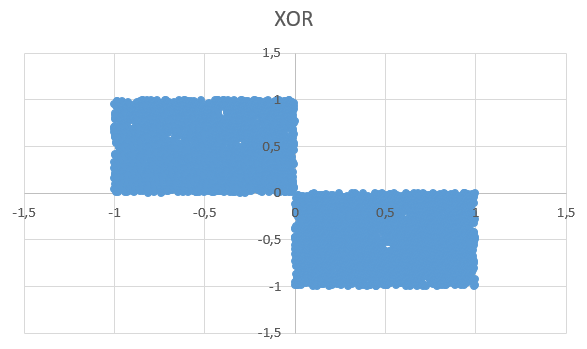
\includegraphics[scale=0.5]{images/resultat_xor.png}
  \caption{Résultat d'un XOR sur $1000$ tests après $10000$ apprentissages pour un réseau 2-2-1}
\end{figure}
